\documentclass[a4paper,11pt]{article}

\usepackage{fullpage}
\usepackage[french]{babel}

\usepackage[utf8]{inputenc}
\usepackage[T1]{fontenc}

% Font : (better idea ?)
\usepackage{newpxtext}
\usepackage{newpxmath}

\usepackage{url}
%for images
\usepackage{graphicx}
%for code-quoting
\usepackage{listings}
%for pseudo-code algo
\usepackage{algorithm}
\usepackage{algpseudocode}
% Parameters for listings

\lstset{%
  basicstyle=\footnotesize\sffamily,%
  columns=fullflexible,%
  frame=lb,%
  frameround=fftf,%
  language=caml,%
}%

\begin{document}

\begin{titlepage}
  \title{Tours de Hanoï et Pavage de Penrose}
  \author{Guillaume Barbier, Romain Ferrand}
  \date{\today}

  \maketitle

  \begin{abstract}
    
  \end{abstract}
\end{titlepage}

\section*{Introduction}
\begin{center}
	Dans ce document nous allons vous présenter notre étude du problème de Hanoï,
    ainsi que les différentes implémentations visant à sa résolution.
    Puis étudierons différents pavages de Penrose.
\end{center}

\section{Tours de Hanoï}
\label{chap:hanoi}

\subsection{Présentation du problème}
\label{sec:prezHanoi}
\begin{figure}
  \centering
  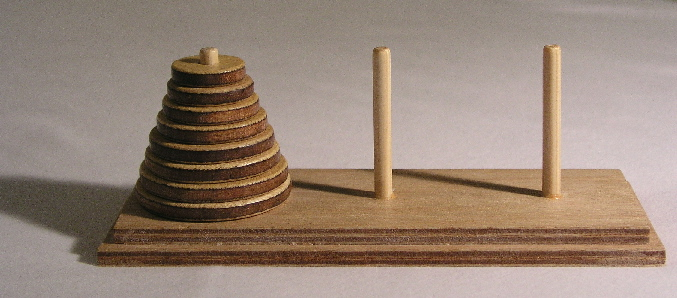
\includegraphics[width=0.8\textwidth]{Tower_of_Hanoi.jpeg}
  \caption{Evanherk wikipédia}
  \label{fig:phd}
\end{figure}

Les Tours de Hanoï est un jeu de réflexion inventé par le mathématicien \textbf{Édouard Lucas} (1842-1891).
Il consiste à déplacer un nombre donné de disques de différents diamètre de la tour de départ vers la tour d'arriver,
tout en passant par une tour intermédiaire.

Le joueur doit également respecter deux règles:
\begin{itemize}
\item déplacer un disque à la fois;
\item ne pas déplacer un disque donné sur un disque plus petit.
\end{itemize}

\subsubsection{Implémentation sans affichage graphique}
\label{sec:algoBase}
L'algorithme le plus intuitif pour résoudre le problème des Tours de Hanoï à trois tours,
est un algorithme récursif très simple.

\begin{algorithm}
  \caption{Tours de Hanoï}\label{algo:hanoi1}
  \begin{algorithmic}[1]
    \Procedure{Hanoi}{$disque,src,aux,dest$} \Comment{Trois tours : source, auxiliaire et destination}
    \If{$disque = 0$}
    ne rien faire
    \Else
    \State Hanoi ($disque - 1, src, dest, aux$)
    \State déplacer \textbf{disque} de \textbf{src} à \textbf{dest}
    \State Hanoi ($disque - 1, aux, src, dest$)
    \EndIf
    \EndProcedure
\end{algorithmic}
\end{algorithm}
Il a donc été sans trop difficulté implémenté, avec, dans un premier temps,  un affichage console pour signifier les mouvements effectués.
\begin{lstlisting}
  let rec hanoi (nb_disc:int) (a:rod) (b:rod) (c:rod) =
    if nb_disc = 0 then ()
    else
      begin
        hanoi a c b (n_disc-1);
        movement a c;
        hanoi b a c (n_disc-1)
      end
  ;;
\end{lstlisting}

\subsubsection*{Bilan 1ère implémentation et retour sur le code}%trouver un truc moins long
Comme expliqué précèdement l'implémentation basique de Hanoï étant assez simple aucunes réelle difficulté n'a été relevée.
Nous avons simplement défini un tour par un nouveau type \textbf{rod}, qui dans cette première implémentation est une lettre.
Lors de la première évaluation du code, il nous a été demandé d'utiliser le \emph{patter matching} de \textbf{Ocaml} que lorsque
cela le justifiait.
La procédure Hanoï ne justifiant pas son utilisation, puisqu'elle peut être remplacée par un simple \textbf{if-else},
elle a été changé en conséquence.

\subsection{Implémentation avec affichage graphique}
Dans le cas des tours de Hanoï, nous avons implémenté la première extension proposée à savoir un affichage graphique.
Dans notre implémentation nous avons souhaité afficher à la fois les piquets et les disques.

Notre première approche a été de considérer les types suivants :
\begin{description}
\item[type :] Disque 
	\begin{itemize}
	\item hauteur
	\item largeur 
	\end{itemize}
\item[type :] Contenu piquet
	\begin{itemize}
	\item liste de disque
	\end{itemize}
\item[type :] Forme piquet
	\begin{itemize}
	\item couleur
	\item rectangle (4 points) 
	\end{itemize}
\item[type :]Position piquet
	\begin{itemize}
	\item point 
	\end{itemize}
\item [type :] Piquet 
	\begin{itemize}
	\item position
	\item forme
	\item contenu 
	\end{itemize}
\end{description}

Les disques comme ayant une relation de combinaison avec les piquets, ainsi chaque piquet "possède" sa pile de disque et l'affiche en fonction de sa position.
l'idée étant de gérer le déplacement donné par l'algorithme de Hanoï par un pop du piquet source en push du piquet destination, et de gérer par la suite l'affichage piquet par piquet. 

Dans un premier temps, nous avons implémenté ces types sous forme de tuples, cette manière de faire à rapidement crée un code lourd et complexe à gérer.
En effet, dans le cas du type \textbf{Piquet}, nous devions reflèchir de manière positionelle ou utiliser l'unpacking de Ocaml, tout en utilisant à la fois que la partie du tuple qui était nécéssaire, nous avions donc a traité plus de données que nous en avions besoin.
Dans un même temps le "champ" \textit{contenu} du type \textbf{piquet} était immutable,
cela se caractèrisait par la nécéssité de reconstruire une instance de \textbf{piquet} à chaque modification de sa liste de disque.

Nous avons donc décidé de remplacer le tuple de \textbf{piquet} par un record, tout en rendant mutable le champ contenu.
Cette manière de faire à permis de clarifier énormément le code, puisque grâce à l'opérateur de résolution de portée ".", nous avions un moyen simple de spécifier le lien entre les données.
Cela a permit également de simplifier le code, puisque nous avions plus besoin de réfléchir en terme de position ou d'unpacking, et la liste mutable de disque nous permetait de ne pas avoir à recrée des instances de type \textbf{piquet}.


\subsubsection{retour sur le code}
Après l'évaluation du code il nous a été demandé de privilègier un code modulable.
Un module Rod (piquet) à donc été crée.
Dans sa signature se module permet de crée des piquet, toutes les stuctures auxiliaires qu'il 
et gère également l'affichage des structures.
Ce module permet de gérer les données de manière abstraite dans le code principale, ainsi même si notre implémentation, gère la forme du piquet et sa position comme des tuples ainsi que son contenu comme une liste de disque, cette concidèration est interne, non visible à l'utilisateur et générique.

Optimisation possible de l'affichage :
Notre implémentation va a chaque mouvement, nettoyer la fenêtre et tout réafficher.
Si cette implémentation du code semble peu optimale par rapport à un remplacement par un carré rectangle sur la précédente position du disque.
Elle se justifie par la présence des piquets, qui nécéssite donc l'affichage d'un deuxième rectangle de la bonne couleur en fonction du piquet, mais également par le fait que cette optimisation ne justifie sans doute pas la complexification du code au regard de la simplicité des opérations effectuées.

Une seconde optimisation cette fois effectué a été d'utiliser le double buffering du module Graphics:
Graphics par défaut "dessine" à la fois sur l'écran et dans une zone mémoire appelé backing store.
Grâce à l'option \textbf{autosynchronize false}.
Nous avons pu faire en sorte que graphics écrive que dans le "backing store" et qu'il se synchronise avec l'affichage que lorsqu'on le juge utile, à savoir lorsque toutes les opérations d'affichage ont été effectuées.
Cette manière de faire permet d'éviter les problèmes de \textit{flickering} même lorsque la vitesse du jeu est très rapide.

Modification de type forme :
Lors de la précédente implémentation le type \textbf{forme piquet} à été conçu comme un tuple d'une couleur et de 4 points, cette représentation est différente du type de \textbf{disque} sans que cela se justifie.
En effet comme nous stockons la position des piquets il aurait été redondant de stocker les points de la forme du piquet calculer en fonction de cette position.
Nous avons donc juger utile de ne garder que sa position, sa hauteur et sa largeur.

\end{document}